\documentclass[11pt]{article}

\renewcommand\familydefault{\sfdefault}
\usepackage[left=3cm,right=3cm,top=2cm,bottom=3cm]{geometry}

% graphics, colors & math
\usepackage{graphicx}
\usepackage[dvipsnames,usenames]{xcolor}
\usepackage{amsmath,amsfonts,nicefrac,textcomp,icomma,bm}

% links & figures
\usepackage{hyperref}
\usepackage[labelfont=bf,font=small]{caption}
\captionsetup[figure]{font={stretch=1}}
\newcommand{\bcaption}[2]{\caption[#1]{\textbf{#1} #2}}

% cross-referencing
\usepackage{xr}
\makeatletter
\newcommand*{\addFileDependency}[1]{%
  \typeout{(#1)}
  \@addtofilelist{#1}
  \IfFileExists{#1}{}{\typeout{No file #1.}}
}
\makeatother

\usepackage{pdfpages}

% line spacing
\usepackage{setspace}
\renewcommand{\baselinestretch}{1.5}
\setlength{\parindent}{2em}

% line numbering
\usepackage{etoolbox,lineno}
\newcommand*{\Section}[1]{\par\nolinenumbers\section*{#1}\linenumbers}

% title layout
\usepackage[affil-it]{authblk}
\renewcommand\Authands{ \& }

\usepackage{lipsum}
\makeatletter
\renewcommand{\maketitle}{\bgroup
\setlength{\parindent}{0pt}\begin{flushleft}
\textbf{\Large{\@title}}\\\vspace{1em}\@author
\end{flushleft}\egroup}
\makeatother

\author[1,2,3]{Pierre-Luc Germain}
\author[1,2]{Anthony Sonrel}
\author[1,2]{Mark D. Robinson}

\affil[1]{Department of Molecular Life Sciences, University of Z{\"u}rich, Switzerland}
\affil[2]{SIB Swiss Institute of Bioinformatics, Z{\"u}rich, Switzerland}
\affil[3]{D-HEST Institute for Neuroscience, Swiss Federal Institute of Technology (ETH), Z{\"u}rich, Switzerland}

\date{\today}

% code font-style
\newsavebox{\foobox}
\newcommand{\slantbox}[2][0]{\mbox{%
        \sbox{\foobox}{#2}%
        \hskip\wd\foobox
        \pdfsave
        \pdfsetmatrix{1 0 #1 1}%
        \llap{\usebox{\foobox}}%
        \pdfrestore
}}
\newcommand\unslant[2][-.25]{\slantbox[#1]{$#2$}}
\newcommand{\code}[1]{\unslant{\mathit{#1}}}

% citations
\usepackage[style=nature,citestyle=numeric,sorting=none]{biblatex}
\renewcommand*{\bibfont}{\footnotesize}
\addbibresource{refs.bib}

\renewcommand{\cite}[1]{\textcolor{Blue}{$^[$\supercite{#1}$^]$}}
\newcommand{\citet}[1]{\citeauthor{#1}\textcolor{Blue}{$^[$\supercite{#1}$^]$}}

% check marks
\usepackage{pifont}
\newcommand{\cmark}{\textcolor{Green}{\ding{51}}}
\newcommand{\xmark}{\textcolor{Red}{\ding{55}}}

% tables
\usepackage{colortbl}


\title{\textit{pipeComp}: A framework for pipeline benchmarking and its application to single-cell RNAseq clustering}

\begin{document}

\thispagestyle{empty}
\maketitle

\linenumbers
%\modulolinenumbers[5]

\Section{Abstract}

The massive growth of single-cell RNA sequencing (scRNAseq) and methods for its analysis still lacks sufficient and up-to-date benchmarks that would guide analytical choices. Moreover, current studies are often focused on isolated steps of the process. Here, we present a flexible R framework for pipeline comparison with multi-level evaluation metrics, and apply it to the benchmark of scRNAseq analysis pipelines using datasets with known cell identities. We evaluate common steps of such analyses, including filtering, doublet detection (suggesting a new R package, \textit{scDblFinder}), normalization, feature selection, denoising, dimensionality reduction and clustering. On the basis of these analyses, we make a number of concrete recommendations about analysis choices. The evaluation framework, \textit{pipeComp}, has been implemented so as to easily integrate any other step or tool and permit extensible benchmarks (\url{https://github.com/plger/pipeComp}). 

\newpage
\pagenumbering{arabic}








\clearpage
\singlespacing
\nolinenumbers
\printbibliography

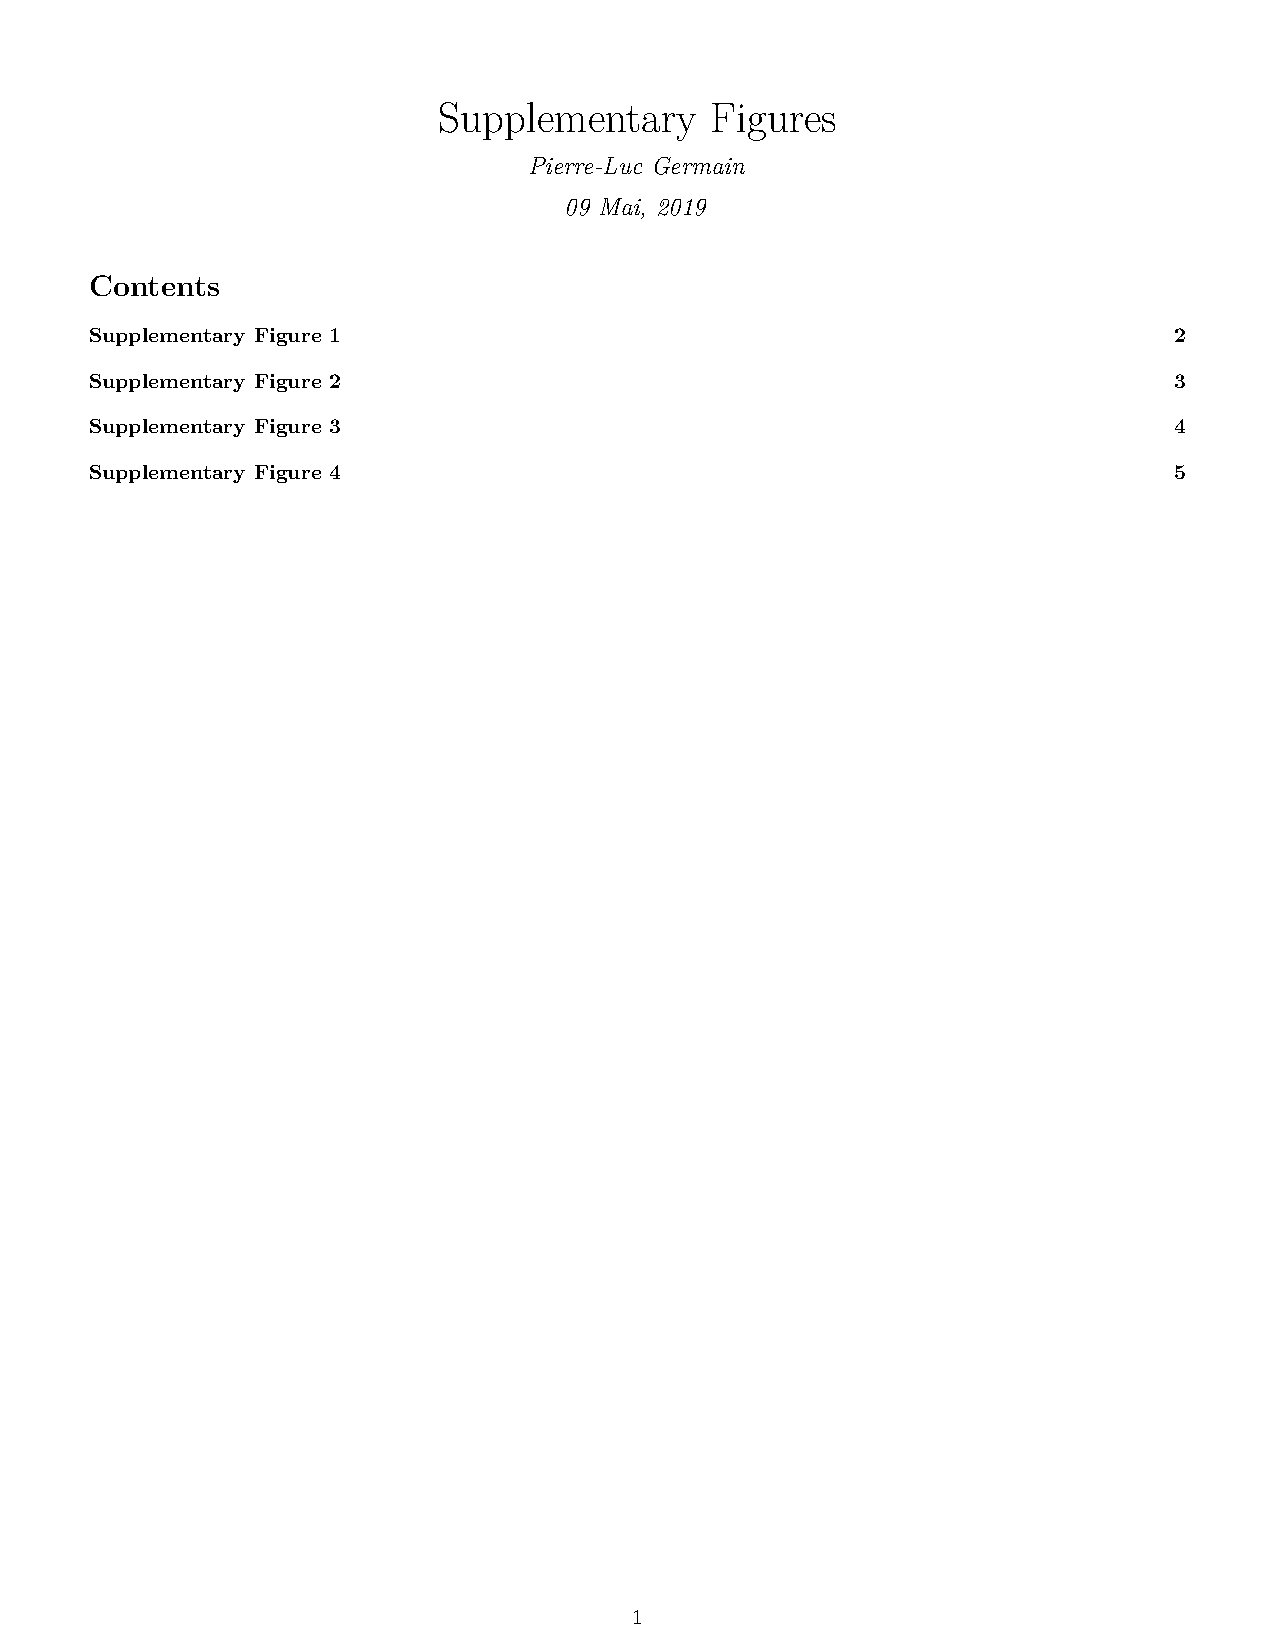
\includepdf[pages=-]{supplementary_figures/supp_figures.pdf}

\end{document}